At \stage{4}, the independent \rvs, power model, and thermal model are fused together under the desired workload, $\profilePdyn$, to produce the corresponding stochastic power $\profileP{\o}$ and temperature $\profileT{\o}$ profiles. The obtained stochastic profiles are nothing more than two polynomials of $\Z_1(\o)$ and $\Z_2(\o)$ with time-dependent coefficients.

The construction of PC expansions is based on the Hermite basis (see \tref{askey}) as it was found to be optimal in situations involving Gaussian parameters \cite{xiu2010}.
A one-dimensional example of the basis is given in \fref{hermite} where the first six Hermite polynomials $\{ \pcb_i(\z) \}_{i = 1}^6$ are displayed.

In two dimensions, assuming a second-total-order PC expansion, the temperature at the $k$th moment of time is
\begin{align*}
  \vTO_k(\o) &= \pccs_{k1} + \pccs_{k2} \Z_1(\o) + \pccs_{k3} \Z_2(\o) + \pccs_{k4} \Z_1(\o) \Z_2(\o) \\
  & \qquad \qquad {} + \pccs_{k5} (\Z_1(\o)^2 - 1) + \pccs_{k6} (\Z_2(\o)^2 - 1)
\end{align*}
where $\pccs_{ki}$ are vectors with two elements corresponding to the two processors.

Once the basis has been chosen, we need to compute the corresponding coefficients, specifically, $\pcc{\vP}_i$ in \eref{pc-expansion}. As shown in \aref{polynomial-chaos}, the computation of $\pcc{\vP}_i$ involves multidimensional integration with respect to the \pdf\ of the \rvs\ $\vZ(\o)$.
In numerical analysis, this task is typically accomplished by virtue of a quadrature rule \cite{press2007}, which, loosely speaking, is a weighted summation over the integrand values computed at prescribed points. A natural choice of a quadrature rule when the weight function is a Gaussian \pdf\ is the Gauss-Hermite quadrature. Further details are given in \aref{gauss-quadrature}.

To summarize, we have completed four out of five stages of the proposed UQ framework depicted in \fref{algorithm}. The result is a light surrogate of the model in \eref{fourier-system}. At each moment of time, the surrogate is composed of two $\nprocs$-valued polynomials, one for power and one for temperature, that are defined in terms of $\nvars$ mutually independent \rvs; an example of such a polynomial is given in \eref{pc-k}. The constructed representation can be trivially analyzed to retrieve various statistics of the system in \eref{fourier-system}, and this is \stage{5}\ in \fref{algorithm}, which will be illustrated as a part of the next section.

\begin{figure}
  \centering
  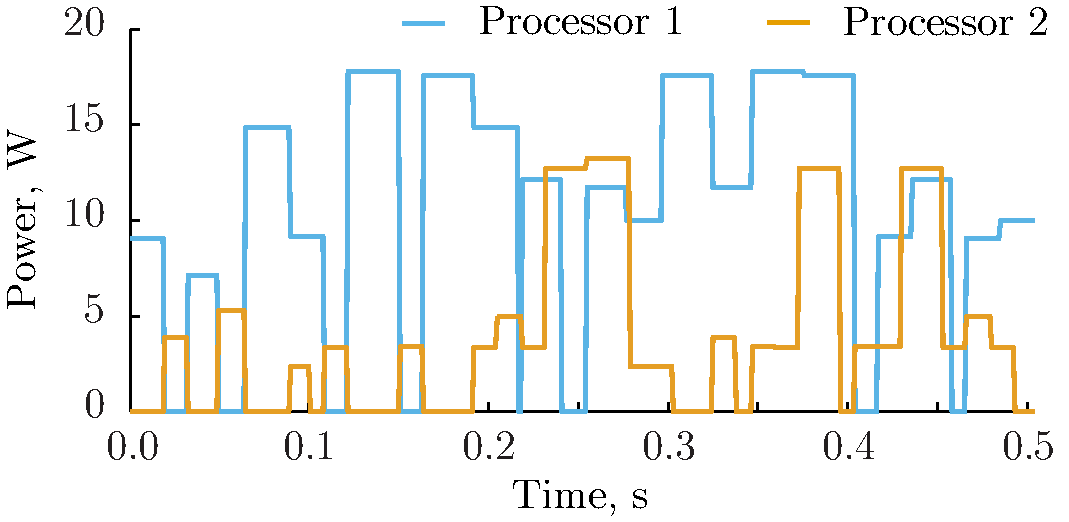
\includegraphics[width=1.00\columnwidth]{include/assets/application-power.pdf}
  \vspace{-0.5em}
  \caption{A dynamic power profile.}
  \flabel{application-power}
  \vspace{-0.5em}
\end{figure}

Assume that the dynamic power profile, $\profilePdyn$, corresponding to the considered workload is the one shown in \fref{application-power}.

\begin{figure}[bl]
  \vspace{-1.0em}
  \centering
  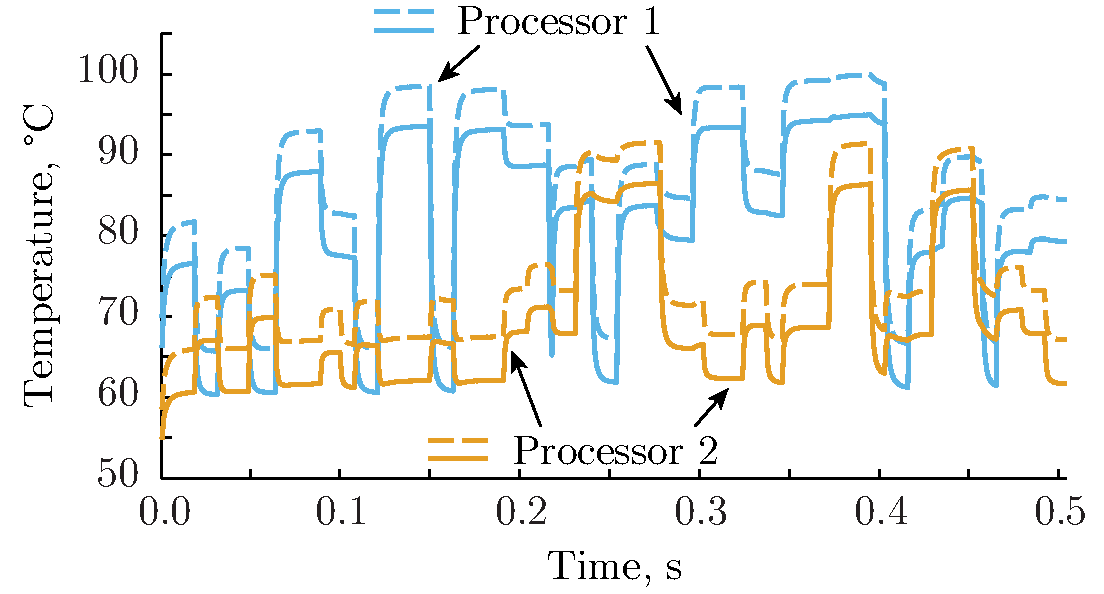
\includegraphics[width=0.90\columnwidth]{include/assets/application-temperature.pdf}
  \vspace{-0.5em}
  \caption{The expected temperature (the solid lines) and one standard deviation above it (the dashed lines).}
  \flabel{application-temperature}
\end{figure}

The expansion for power has the same structure but different coefficients.
Such a series might be shorter or longer depending on the accuracy requirements.
As we see, our surrogate model has a negligibly small computational cost to undertake UQ at \stage{5}: for any outcome of the uncertain parameters $\vZ(\o) \equiv \vZ$, we can easily compute the corresponding temperature by plugging $\vZ$ into the above equation; the same applies for power.
Thus, such characteristics as \cdfs\ and \pdfs\ (see \fref{motivation-pdf}) can be rigorously estimated. Furthermore, the expectation and variance at the $k$th moment of time are calculated as simply as
\[
  \oExp{\vTO_k(\o)} = \pccs_{k1} \hspace{1em} \text{and} \hspace{1em} \oVar{\vTO_k(\o)} = \sum_{i = 2}^{6} \pcn_i \: \pccs_{ki}^2
\]
where $\pcn_i$ are normalization constants, and the squaring should be understood element-wise.
For the nominal power profile $\profilePdyn$ depicted in \fref{application-power}, we obtain the corresponding stochastic temperature profile $\profileT{\o}$ and can observe, \eg, its expectation and standard deviation; they are plotted in \fref{application-temperature}.
The displayed curves closely match those obtained via MC simulations with $10^4$ samples; however, our method takes less than a second, on a personal laptop, while MC sampling takes more than a day, which we discuss in \sref{experimental-results}.
